\def\modulename{pcp}
\RequirePackage[utf8]{course}
\pcp
\newif\ifsolution
\solutionfalse

\usepackage{caption}
\usepackage{subcaption}
\usepackage{units}
\usepackage{listings}
\usepackage{Cdefs}
\usepackage{tikz}
\usetikzlibrary{arrows}

\tikzset{
  treenode/.style = {align=center, inner sep=0pt, text centered,
    font=\sffamily},
  arn_n/.style = {treenode, circle, white, font=\sffamily\bfseries, draw=black,
    fill=black, text width=1.5em},% arbre rouge noir, noeud noir
  arn_r/.style = {treenode, circle, red, draw=red, 
    text width=1.5em, very thick},% arbre rouge noir, noeud rouge
  arn_x/.style = {treenode, rectangle, draw=black,
    minimum width=0.5em, minimum height=0.5em}% arbre rouge noir, nil
}

\def\consigne#1{\null\begin{center}\parbox{13cm}{\large #1}\end{center}\relax}

\def\Question#1#2{\question{}\textbf{(#2)} #1}
\ifsolution
\includecomment{solution}
\else
\excludecomment{solution}
\fi

\begin{document}
\controlecontinu

\consigne{{\bf Dur{\'e}e: 1h30. Aucun document n'est autorisé.}}

\begin{solution}
  Note de l'auteur: les solutions proposées sont complètes (de mon
  point de vue) et sont écrites pour être compréhensibles avec les
  rappels de cours qui vont avec. Il n'est pas nécessaire d'écrire
  toutes les étapes pour avoir les points, ni même d'avoir le bon
  résultat: juste savoir ou expliquer comment il aurait fallu faire
  est récompensé.
\end{solution}

\vspace*{1em}

\exo{Codage (4 points)}

\begin{solution}
  Note de l'auteur: cet exercice était un peu trop long par rapport
  aux points (seulement 4).  Pour l'année prochaine (au cas où cette
  correction circulerait), il y aurait probablement plus de points sur
  cette partie, avec le même type de questions.
\end{solution}


On rappelle qu'un nombre:
\[
x=(-1)^s\cdot 2^{e-127}\cdot (1+\frac M{2^{23}})
\]
est codé sous la forme:
\begin{center}
  \begin{tabular}{|c|c|c|}
    \multicolumn 1c 0& \multicolumn 1c{\hbox to 8em{1\hfill 8}}&  \multicolumn 1c{\hbox to 23em {9\hfill 31}}\\
    \hline
    s &  e & M \\
    \hline
  \end{tabular}
\end{center}

\question (2 pts) Donnez le code hexadécimal du signe \(s\), de l'exposant \(e\), et de la mantisse \(M\), ainsi que le code entier sur 32 bits, du nombre \(-10,5\).

\begin{solution}
  On a:
  \begin{eqnarray*}
    -10,5&=&(-1)^1\cdot 2^3\cdot (1 + \frac{2,5}{8})\\
         &=& (-1)^1\cdot 2^{130-127}\cdot (1 + \frac{5}{16})\\
         &=& (-1)^1\cdot 2^{130-127}\cdot (1 + \frac{5}{2^4})\\
         &=& (-1)^1\cdot 2^{130-127}\cdot (1 + \frac{5\cdot 2^{19}}{2^{23}})\\
  \end{eqnarray*}
  Donc:
  \[
    s = 1 \hspace*{3em}e=130\hspace*{3em}M=5\cdot 2^{19}
  \]
  En base 16 (hexadécimal):
  Donc:
  \[
    s = 1 \hspace*{3em}e=128+2=82\hspace*{3em}M=5\cdot 8\cdot 2^{16}=280000
  \]
  Pour écrire en binaire le code entier, on écrit tout en base 2:
  \[
    \overbrace{\underbrace{1}_1}^s\,\,
    \overbrace{\underbrace{1000}_8\,\underbrace{0010}_2}^e\,\,
    \overbrace{\underbrace{010}_2\,\underbrace{1000}_8\,\underbrace{0000}_0\,\underbrace{0000}_0\,\underbrace{0000}_0\,\underbrace{0000}_0}^{M\text{ sur 23 bits}}
  \]
  et on regroupe par groupe de 4, qu'on traduit en hexadécimal:
  \[
    \underbrace{1100}_{12=C}\,\underbrace{0001}_1\,\underbrace{0010}_2\,\underbrace{1000}_8\,\underbrace{0000}_0\,\underbrace{0000}_0\,\underbrace{0000}_0\,\underbrace{0000}_0
  \]
  Donc le code entier en hexadécimal est \(C1280000\).
\end{solution}
\question (2 pts) On utilise la méthode par multiplications
successives (en base 16). 


\begin{solution}
  Pour avoir 10 chiffres en base 2, il en faut 3 en base 16 (et on
  aura une estimation trop précise ayant 12 chiffres en base 2):
  \begin{eqnarray*}
    0,23 \cdot 16 &=& \fbox{3},68\\
    0,68\cdot 16 &=& \fbox{10},88\\
    0,88\cdot 16 &=& \fbox{14},08\\
  \end{eqnarray*}
  Donc:
  \begin{eqnarray*}
    1,23 &=& (1,3AE)_{16}\\
    &=&(1,0011\,1010\,1110)_2\\
    &=&\fbox{\((1,0011\,1010\,11)_2\)}\hspace*{2em}\text{avec 10 chiffres significatifs}\\
  \end{eqnarray*}
  
\end{solution}

\exo{Test de compréhension (4 points)}

\begin{center}
  \fbox{~\parbox{0.9\textwidth}{%
      Comme cela n'a pas été beaucoup vu en TP, on rappelle que si \(x\) est une valeur, alors:
      \begin{center}
        \texttt{( t ) x}
      \end{center}
      est la traduction de cette valeur dans le type \texttt{t}.
    }~}
\end{center}

On considère la fonction \texttt{main} suivante:

\begin{lstlisting}[language=C]
int main ( int argc , char * argv[] )
{
  int t[3] = {1,2,3} ;
  int * p1 = ( int * ) ( t + 1 ) ;
  int * p2 = ( int * ) ( & t + 1 ) - 1 ;
  * ( t + 2 ) = p1 [ 1 ] - t [ 0 ] ;
  p2[-2] = p1[1] ;
  printf ( "%d %d %d\n" , t[0] , t[1] , t[2] ) ;
  return 0 ;
}
\end{lstlisting}

\question (2 points) Expliquez, en vous aidant si possible de schémas,
quelles sont les valeurs, en tant qu'entier, de \(p_1\) et \(p_2\) en
fonction de la valeur de \(t\) en tant qu'entier. Pour simplifier, on
suppose que \texttt{sizeof ( int ) = 4}.

\begin{solution}
  Il est nécessaire (et suffisant) de faire un schéma de la mémoire pour s'y retrouver !
  Au début, on a:
  \begin{center}
    \begin{tabular}{|c|c|c|c|c|}
      \multicolumn 1l{100}&\multicolumn 1l{104}&\multicolumn 1l{108}&\multicolumn 1l{112}&\multicolumn 1l{116}\\
      \hline
      1&2&3&& \\
      \hline
      \multicolumn 1c{t[0]}&\multicolumn 1c{t[1]}&\multicolumn 1l{t[2]}&\multicolumn 1l{p1}&\multicolumn 1l{p2}\\
      \multicolumn 3c{\upbracefill}&\multicolumn 2c{}\\
      \multicolumn 3c{t}&\multicolumn 2c{}\\
    \end{tabular}
  \end{center}
  Pour les additions et soustractions sur les adresses en tant
  qu'entier, si \(x\) est l'adresse d'une valeur de type \texttt{t}, alors
  en tant qu'entier, \(x+1\) vaut \texttt{x + sizeof ( t )}.
  \begin{enumerate}
  \item \texttt{t} est l'adresse de \texttt{t[0]}, une valeur de type
    \texttt{int}, donc \texttt{t+1} vaut en tant qu'entier \texttt{t +
      sizeof ( int )}, soit \texttt{104} sur le schéma (c'est défini
    ainsi pour que \texttt{t+1} soit l'adresse de \texttt{t[1]});
  \item \texttt{\& t} est l'adresse de \texttt{t}, une
    valeur qui est un tableau de 3 entiers, donc
    \texttt{\& t+1} vaut en tant qu'entier \texttt{t + 3 *
      sizeof ( int )}, soit \texttt{112} sur le schéma. On traduit
    ensuite cette valeur en tant qu'adresse d'un entier, et on enlève 1, donc en tant qu'entier on obtient l'adresse \texttt{112 - sizeof ( int )=108}.
  \end{enumerate}
  Donc après l'initialisation, on a:
  \begin{center}
    \begin{tabular}{|c|c|c|c|c|}
      \multicolumn 1l{100}&\multicolumn 1l{104}&\multicolumn 1l{108}&\multicolumn 1l{112}&\multicolumn 1l{116}\\
      \hline
      1&2&3&104&108 \\
      \hline
      \multicolumn 1c{t[0]}&\multicolumn 1c{t[1]}&\multicolumn 1l{t[2]}&\multicolumn 1l{p1}&\multicolumn 1l{p2}\\
      \multicolumn 3c{\upbracefill}&\multicolumn 2c{}\\
      \multicolumn 3c{t}&\multicolumn 2c{}\\
    \end{tabular}
  \end{center}
  On passe ensuite à l'évaluation des 2 instructions:
  \begin{itemize}
  \item \texttt{t[2] = * ( p1 + 1 ) - t[0]}. D'après ce qui précède,
    \texttt{p1+1} est l'adresse de \texttt{t[2]}, donc on pourrait
    écrire de manière plus simple: \texttt{t[2] = t[2] - t[0]=2};
  \item \texttt{p2[-2] = t[2]}. D'après ce qui précède, \texttt{p2-2}
    est l'adresse d'une case contenant un entier 2 cases contenant des
    entiers avant \texttt{t[2]}, donc on pourrait écrire de manière
    plus simple: \texttt{t[0] = t[2] =2};
  \end{itemize}
  Donc avant le \texttt{printf}, le contenu de la mémoire est:
  \begin{center}
    \begin{tabular}{|c|c|c|c|c|}
      \multicolumn 1l{100}&\multicolumn 1l{104}&\multicolumn 1l{108}&\multicolumn 1l{112}&\multicolumn 1l{116}\\
      \hline
      2&2&2&104&108 \\
      \hline
      \multicolumn 1c{t[0]}&\multicolumn 1c{t[1]}&\multicolumn 1l{t[2]}&\multicolumn 1l{p1}&\multicolumn 1l{p2}\\
      \multicolumn 3c{\upbracefill}&\multicolumn 2c{}\\
      \multicolumn 3c{t}&\multicolumn 2c{}\\
    \end{tabular}
  \end{center}  
  Le programme affiche \texttt{2 2 2}.

   
\end{solution}


\begin{solution}
  Note de l'auteur: On a fait ce genre de schéma en cours et en TP. Il
  est \textbf{très important} de bien les comprendre. On a dans cet
  exercice tout ce qui est difficile dans la programmation en C, le
  reste est simple.
\end{solution}

\exo{Somme des éléments d'un tableau (4 points)}

\begin{solution}
  Note de l'auteur: après 2 exercices relativement difficiles, un
  exercice normalement simple. J'écris ces lignes avant d'avoir
  corriger les copies du CC1\(\ldots\) Il y a en particulier un
  guidage maximum sur ce qu'il faut écrire, ce ne sera pas toujours le
  cas !
\end{solution}

On veut écrire une fonction \texttt{somme\_partielle} qui prend en
entrée l'adresse de la première case d'une tableau d'entiers, le
nombre \(n\) de cases de ce tableau, un entier \(i\) qui devrait être
l'indice d'une case dans le tableau, et l'adresse d'une variable (de
type \texttt{int}) dans laquelle il faudra stocker:
\[
\Sigma_{j=0}^i t[j]
\]
c'est-à-dire la somme des éléments du tableau de l'indice 0 à l'indice
\(i\) (inclus). Cette fonction renvoie \(0\) si le calcul est
possible, et \(1\) sinon.

\question (1 point) Donnez la déclaration de cette fonction.
\begin{solution}
  \begin{lstlisting}[language=C]
    int somme_partielle ( int * t , int n , int i , int  * resultat ) ;
  \end{lstlisting}
\end{solution}

\question (0,5 points) Décrivez avec une expression C les cas
d'erreur.
\begin{solution}
  Il y a une erreur si \(i\) n'est pas l'adresse d'une case dans le tableau:
  \begin{lstlisting}[language=C]
    ( i < 0 ) || ( i >= n )
  \end{lstlisting}
\end{solution}

\question (2,5 points) Écrivez la fonction.

\begin{solution}
  \begin{lstlisting}[language=C]
int somme_partielle ( int * t , int  n , int i , int * resultat )
{
  int j , somme ;
  if ( ( i < 0 ) || ( i >= n ) )
    return 1 ;
  for ( j = 0 , somme = 0 ; j <= i ; j++ )
    somme = somme + t[j] ;
  * resultat = somme ;
  return 0 ;
}
  \end{lstlisting}
\end{solution}

\exo{Tas (8 points)}

\begin{solution}
  Note de l'auteur: Il y a beaucoup plus à lire et comprendre qu'à
  écrire dans cet exercice ! \c Ca arrive souvent quand il faut écrire
  un programme.
\end{solution}

\paragraph{Pr{\'e}liminaires.}
Un \emph{arbre} est soit un arbre vide, soit est un n\oe{}ud (la
\emph{racine} de cet arbre) qui est le p{\`e}re de deux \emph{fils}, son
fils droit et son fils gauche, qui sont eux-m{\^e}mes des arbres.

Les \emph{tas} sont des tableaux qui codent certains arbres de la
mani{\`e}re suivante:
\begin{itemize}\setlength\itemsep {-3pt}
\item la valeur de la racine de l'arbre est dans la case $0$;
\item si la valeur d'un n\oe ud est stock{\'e}e dans la case $i$, alors
  la valeur de la racine de son fils gauche est stock{\'e}e dans la case
  $2\times i + 1$, et la valeur de la racine de son fils droit est
  stock{\'e}e dans la case $2\times i + 2$;
\item la valeur d'un n\oe ud est toujours plus petite que la valeur
  de ses fils.
\end{itemize}
Pour savoir quand s'arr{\^e}tent les valeurs du tas (les cases blanches de
la Figure~\ref{fig:graph}), on a besoin, en plus du tableau, du nombre
d'{\'e}l{\'e}ments dans le tas. Pour d{\'e}crire des tas en C, on utilise les
d{\'e}clarations suivantes:
\begin{Ccode}
  \ctab\cstruct \ctype{tas\_s} \lb
  \ctab \cint \cvar{nb\_elts} ; \ccomment{nombre d'{\'e}l{\'e}ments dans le tas}
  \ctab \cint * val ; \ccomment{tableau des valeurs}
  \ctab\rb ;
  \ctab\ctypedef \cstruct \ctype{tas\_s} * \ctype{tas} ;
\end{Ccode}

\begin{figure}
  \centering
        \begin{subfigure}[b]{0.5\textwidth}
                \centering
                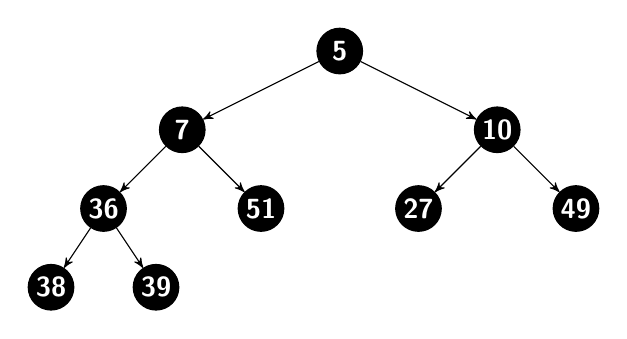
\begin{tikzpicture}[->,>=stealth',level/.style={sibling distance = 4cm/#1,
                    level distance = 1cm}] 
                  \node [arn_n] {5}
                  child{ node [arn_n] {7}
                    child{ node [arn_n] {36} 
                      child{ node [arn_n] {38}}
                      child{ node [arn_n] {39}}
                    }
                    child{ node [arn_n] {51}
                  }
                }
                child{ node [arn_n] {10} 
                    child{ node [arn_n] {27} 
                    }
                    child{ node [arn_n] {49}}                             
                  }
                ; 
                \end{tikzpicture}
                \caption{Un tas, dont la racine a pour valeur $5$, son
                  fils gauche a une racine de valeur $7$ et son fils
                  droit a pour racine un n\oe ud dont la  valeur est 10. Les
                  arbres vides ne sont pas repr{\'e}sent{\'e}s.}
                \label{fig:arbre}
        \end{subfigure}%
        \qquad
        \begin{subfigure}[b]{0.4\textwidth}
                \centering
                %\small
                \begin{tabular}[c]{|c|c|c|c|c|c|c|c|c|c|c|c|}
                  \hline
                  5 & 7 & 10 & 36 & 51 & 27 & 49 & 38 & 39 &  &  &  \\
                  \hline
                  \multicolumn 2l{0} & \multicolumn 3l{2} &
                  \multicolumn 7l {5} \\
                \end{tabular}
                \vspace*{2em}
                \caption{Le tableau correspondant {\`a} ce tas: la valeur
                  de la racine est dans la case $0$, celle de son fils
                droit dans la case $2=2\times 0+2$, et celle du fils
                gauche de ce fils droit est dans la case $5=2\times 2
                + 1$.}
                \label{fig:tableau}
        \end{subfigure}
  \caption{Tas et leur repr{\'e}sentation par un tableau}
  \label{fig:graph}
\end{figure}

\begin{figure}
  \centering
          \begin{subfigure}[b]{0.45\textwidth}
                \centering
                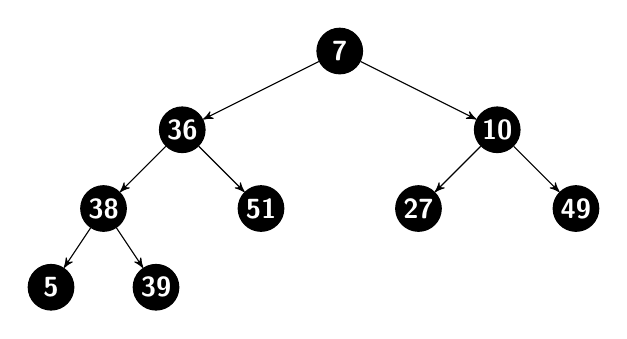
\begin{tikzpicture}[->,>=stealth',level/.style={sibling distance = 4cm/#1,
                    level distance = 1cm}] 
                  \node [arn_n] {7}
                  child{ node [arn_n] {36}
                    child{ node [arn_n] {38} 
                      child{ node [arn_n] {5}}
                      child{ node [arn_n] {39}}
                    }
                    child{ node [arn_n] {51}
                  }
                }
                child{ node [arn_n] {10} 
                    child{ node [arn_n] {27} 
                    }
                    child{ node [arn_n] {49}}                             
                  }
                ; 
                \end{tikzpicture}
                \caption{Le tas de la Figure~\ref{fig:arbre} apr{\`e}s
                  l'{\'e}tape 2 de la suppression.}
                \label{fig:tas:suppression:etape2}
        \end{subfigure}%
        \qquad
          \begin{subfigure}[b]{0.45\textwidth}
                \centering
                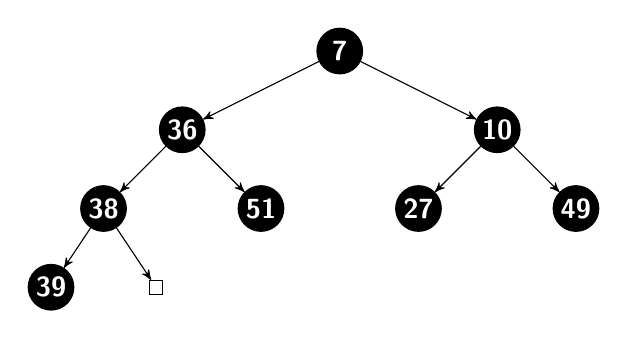
\begin{tikzpicture}[->,>=stealth',level/.style={sibling distance = 4cm/#1,
                    level distance = 1cm}] 
                  \node [arn_n] {7}
                  child{ node [arn_n] {36}
                    child{ node [arn_n] {38} 
                      child{ node [arn_n] {39}}
                      child{ node [arn_x] {}}
                    }
                    child{ node [arn_n] {51}
                  }
                }
                child{ node [arn_n] {10} 
                    child{ node [arn_n] {27} 
                    }
                    child{ node [arn_n] {49}}                             
                  }
                ; 
                \end{tikzpicture}
                \caption{Le tas de la Figure~\ref{fig:arbre} apr{\`e}s
                  l'{\'e}tape 5 de la suppression. Le n\oe ud vide
                  repr{\'e}sente la d{\'e}cr{\'e}mentation du nombre
                  d'{\'e}l{\'e}ments. $39$ est plus grand que $38$, donc
                  l'{\'e}tape 6 ne fait rien}
                \label{fig:tas:suppression:etape5}
        \end{subfigure}%
  \caption{Tas aux diff{\'e}rentes {\'e}tapes de la suppression.}
  \label{fig:tas:suppression:fig}
\end{figure}

\question (0.5 + 0.5 + 1 = 2 pts) {\'E}crire trois fonctions
\cfun{fils\_gauche}, \cfun{fils\_droit}, et \cfun{pere} qui, en
fonction d'un indice $i$, calculent l'indice correspondant
respectivement au fils gauche, au fils droit, et au p{\`e}re du n\oe ud
dont la valeur est stock{\'e}e dans la case $i$. \emph{Par exemple,
  \cfun{pere}(5)=2, et \cfun{fils\_gauche}(2)=5.}

\begin{solution}
  Il faut tester des fonctions simples qui vont bien (on ne demande pas de justifier !):
  \begin{lstlisting}[language=C]
int fils_gauche ( int i )
{
  return 2 * i + 1 ;
}
int fils_droit ( int i )
{
  return 2 * i + 2 ;
}
int pere ( int i )
{
  // on utilise le fait que / est la division entiere
  return ( i - 1 ) / 2 ;
}
  \end{lstlisting}
\end{solution}

\vspace*{1em}

L'algorithme permettant d'ins{\'e}rer un {\'e}l{\'e}ment dans un tas est donn{\'e}
informellement dans la Figure~\ref{fig:tas:insertion}.
\begin{figure}
  \begin{subfigure}[t]{0.45\textwidth}
    \centering
    \fbox{\parbox{\textwidth}{\begin{enumerate}\setlength\itemsep {-3pt}
        \item On note $i$ l'indice courant. Au d{\'e}part, l'indice courant
          est l'indice de la premi{\`e}re case vide dans le
          tableau (dans la Figure~\ref{fig:tableau}, $i$ vaut au d{\'e}part $9$);
        \item mettre l'{\'e}l{\'e}ment {\`a} ajouter dans la case d'indice $i$;
        \item Tant que:
          \begin{itemize}\setlength\itemsep {-3pt}
          \item l'indice courant est strictement positif;
          \item et la valeur du p{\`e}re de l'indice courant est plus grande que
            la valeur de l'indice courant
          \end{itemize}
          {\'e}changer ces deux valeurs, et positionner l'indice courant sur son
          p{\`e}re;
        \item rendre le tas;
        \end{enumerate}}\quad}
    \caption{Algorithme d'insertion d'un {\'e}l{\'e}ment.}
    \label{fig:tas:insertion}
  \end{subfigure}
  \qquad
  \begin{subfigure}[t]{0.45\textwidth}
    \centering
    \fbox{\parbox{\textwidth}{\begin{enumerate}\setlength\itemsep {-3pt}
        \item On note $i$ l'indice courant. Au d{\'e}part, l'indice courant
          vaut $0$;
        \item Tant que le fils droit de l'indice courant est dans le
          tableau:
          \begin{itemize}
          \item {\'e}changer la valeur du n\oe ud courant avec celle du plus
            petit de ses fils;
          \item l'indice courant devient celui du fils avec lequel
            l'{\'e}change a {\'e}t{\'e} fait.
          \end{itemize}
        \item Si l'{\'e}l{\'e}ment courant a un fils gauche, on {\'e}change ces deux
          {\'e}l{\'e}ments, et l'{\'e}l{\'e}ment courant devient l'indice du fils gauche;
        \item on {\'e}change ensuite la valeur de l'{\'e}l{\'e}ment courant et celle
          du dernier {\'e}l{\'e}ment du tas;
        \item on d{\'e}cr{\'e}mente de $1$ le nombre d'{\'e}l{\'e}ments dans le tas;
        \item on remonte, comme pour l'insertion, l'{\'e}l{\'e}ment courant tant
          qu'il est plus petit que son p{\`e}re.  
        \end{enumerate}}\quad}
    \caption{Algorithme de suppression du plus petit {\'e}l{\'e}ment.}
    \label{fig:tas:suppression}
  \end{subfigure}
  \label{fig:tas:algos}
  \caption{Algorithmes sur les tas}
\end{figure}

\question (1 pt) Justifiez (informellement) que l'insertion d'un
{\'e}l{\'e}ment dans un tas permet d'obtenir un tas, \textit{i.e.}, que dans
le tas obtenu, tout {\'e}l{\'e}ment est plus petit que ses fils.

\begin{solution}
  Il suffit de suggérer quelque chose qui ressemble à:
  \begin{itemize}
  \item Avant l'insertion, chaque fils est plus grand que son père;
  \item Après l'insertion, chaque fils sauf celui inséré est plus grand que son père;
  \item Quand le n\oe ud inséré est strictement plus petit que son
    père, on les échange. La seule exception possible devient le
    père. Le nouveau père est strictement plus petit que ses deux fils.
  \item on remonte ainsi jusqu'à ce qu'il n'y ait plus d'exception
    (pas de père/racine, ou fils plus grand que son père
  \end{itemize}
  Le but n'était pas de faire une preuve, mais d'obliger à essayer de
  comprendre pourquoi l'algorithme marche.
\end{solution}

\question (1 pt) De quels arguments (signification de la variable et
son type) est-ce qu'une fonction qui prend en entrée un tas aura
besoin ?

\begin{solution}
  Question faite pour guider. 
  \begin{itemize}
  \item de l'adresse \(t\) de la première case du tableau, de type \texttt{int *};
  \item du nombre \(n\) d'éléments dans le tas (de type \texttt{int}).
  \end{itemize}
\end{solution}

\question (2 pts) {\'E}crire la fonction d'insertion d'un {\'e}l{\'e}ment en C. On suppose
qu'il y a strictement moins d'{\'e}l{\'e}ments dans le tas que le nombre
maximal qu'il ne peut en contenir.

\begin{solution}
  On a besoin du nombre \(n\) d'éléments dans le tas, de la valeur à
  ajouter, et de l'adresse \(t\) de la première case du tas.
  \begin{lstlisting}[language=C]
void insertion ( int * t , int i , int valeur )
{
  int tmp ;
  t[i] = valeur ;
  while ( ( i > 0 ) && ( t[i] < t[ pere(i) ] ) )
  {
    tmp = t[ pere(i) ] ;
    t[ pere(i) ] = t[i] ;
    t[i] = tmp ;
  }
}
  \end{lstlisting}
\end{solution}



\question (2 pts) {\'E}crire la fonction de suppression du plus petit
{\'e}l{\'e}ment en C en se basant sur l'algorithme de la
figure~\ref{fig:tas:suppression}. On suppose qu'il y a au moins un
{\'e}l{\'e}ment dans le tas.

\begin{solution}
  note: il serait exceptionnel que quelqu'un ait tout fait, y compris
  cette question. Un 20, ça se mérite ! Pour en revenir à l'exercice,
  on a besoin de l'adresse de la première case du tableau et de son
  \(n\) d'éléménts.
  \begin{lstlisting}[language=C]
void suppression ( int * t , int n )
{
  int i ;
  int tmp ;
  i = 0 ;
  while ( fils_droit ( i ) < n ) // et donc fils_gauche(i) < n !
  {
    if ( t[ fils_droit ( i ) ] < t[ fils_gauche ( i ) ] )
    {
      tmp = t[fils_droit ( i )] ;
      t[i] = t[fils_droit ( i )] ;
      t[fils_droit ( i )] = tmp ;
      i = fils_droit ( i ) ;
    }
    else
    {
      tmp = t[fils_gauche ( i )] ;
      t[i] = t[fils_gauche ( i )] ;
      t[fils_gauche ( i )] = tmp ;
      i = fils_gauche ( i ) ;
    }
  }
  if ( fils_gauche ( i ) < n )
  {
    tmp = t[fils_gauche ( i )] ;
    t[i] = t[fils_gauche ( i )] ;
    t[fils_gauche ( i )] = tmp ;
    i = fils_gauche ( i ) ;
  }
  t[i] = t[n-1] ;
  while ( ( 0 < i ) && ( t[i] < t[pere(i)] ) )
  {
    tmp = t[pere(i)] ;
    t[pere(i)] = t[i] ;
    t[i] = tmp ;
    i = pere(i) ;
  }
}    
  \end{lstlisting}

  Post-scriptum: on peut simplifier les 2 derniers exercices avec la fonction suivante:
  \begin{lstlisting}[language=C]
void echange ( int * a , int * b )
{
  int tmp ;
  tmp = *a ;
  *a = *b ;
  *b = tmp ;
}    
  \end{lstlisting}
  et utiliser, par exemple:
  \begin{lstlisting}[language=C]
    echange ( t + i , t + pere ( i ) ) ;
  \end{lstlisting}
\end{solution}


\end{document}

